\subsection{Allocation of TCU and RSU }
\label{subsec:allocation_of_tcu_and_rsu}
%%% image process 3 state machine
\begin{figure}[ht]
    \centering
    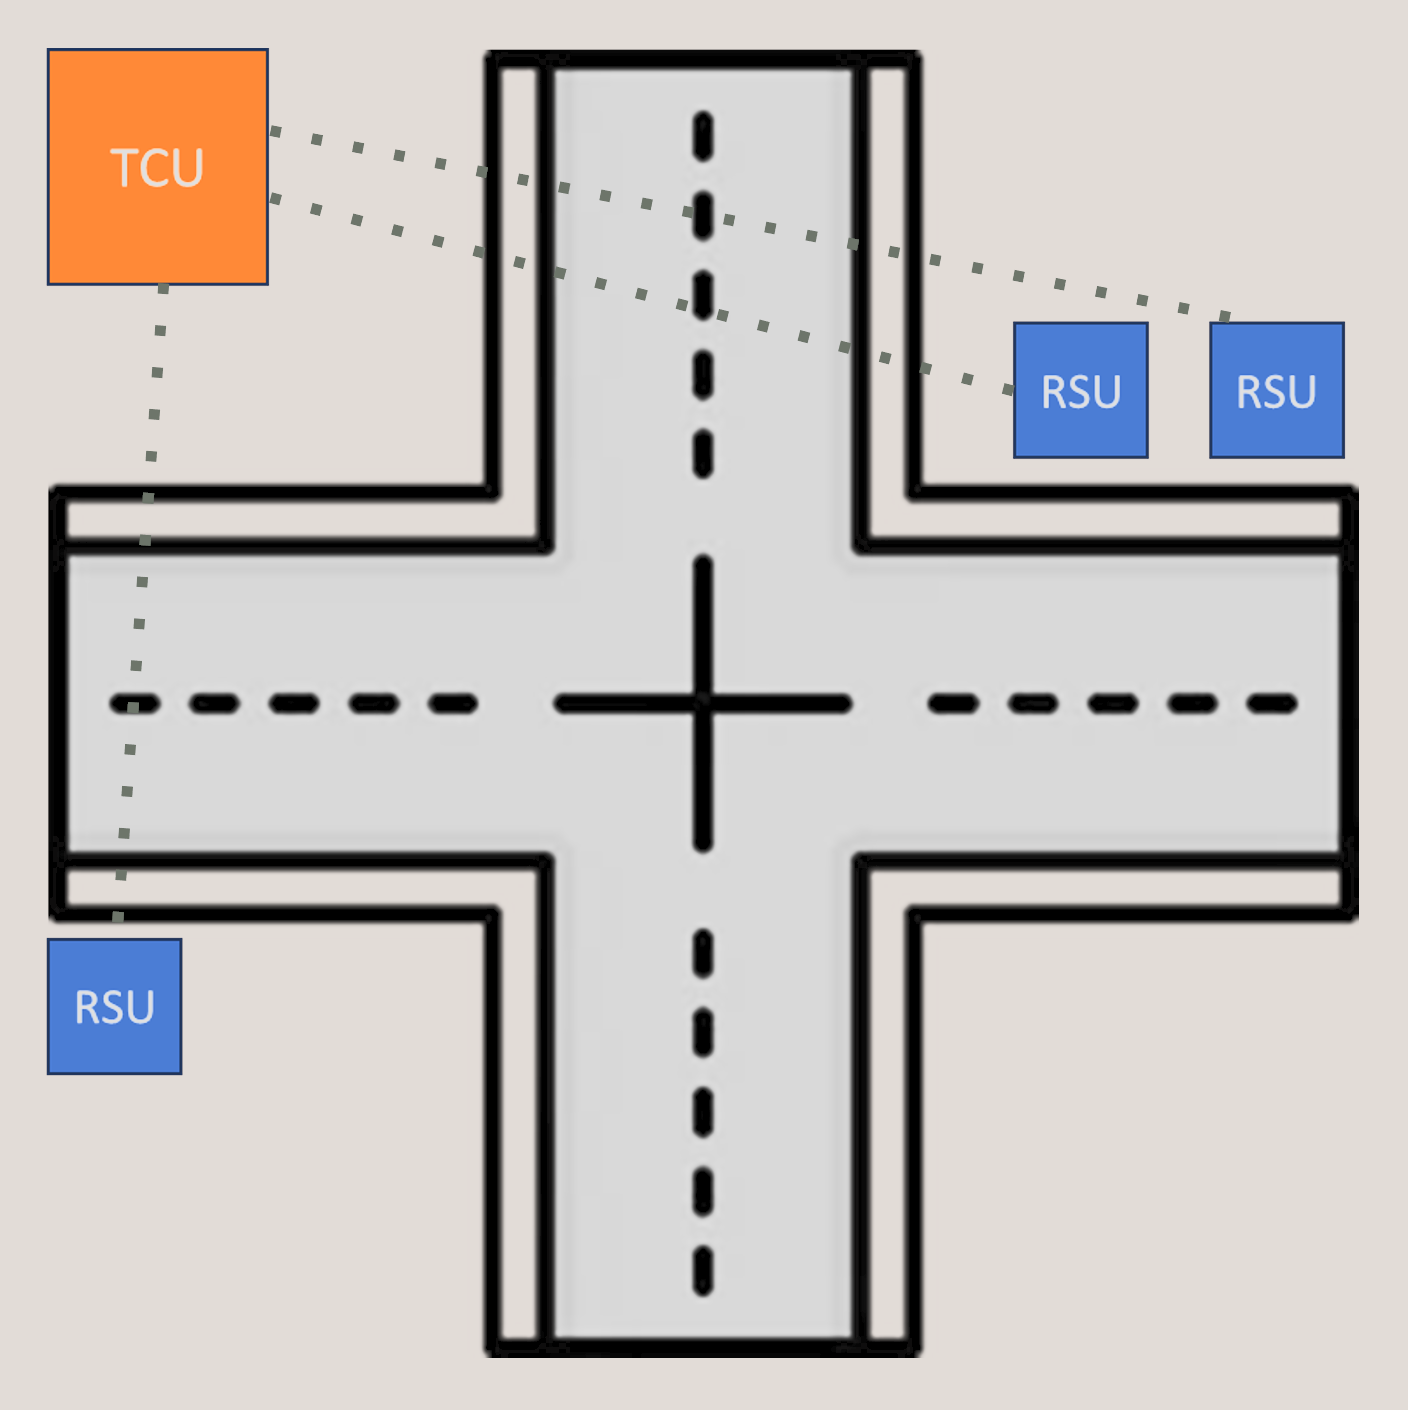
\includegraphics[width=0.3\textwidth]{images/tcu_rsu_position.png}
    \caption{Allocation of TCU \& RSU }
    \label{img:tcu_rcu_position}
\end{figure}
In Figure \ref{img:tcu_rcu_position}, we can see how Traffic Control Unit (TCU) and Roadside Units (RSUs) are positioned to monitor and manage traffic flow. The TCU is a central device that receives and processes data from multiple RSUs, which are devices that are installed at different locations on the roads. The RSUs communicate with vehicles using wireless signals, and collect real-time data such as location, direction, and requested direction etc. The TCU uses this data to analyze the traffic conditions and optimize the traffic signals, speed limits, lane changes, etc. The TCU does not communicate directly with the vehicles, but only with the RSUs. This system can improve traffic safety, efficiency, and environmental impact.
